\documentclass[border=4pt]{standalone}
\usepackage{tikz}\usetikzlibrary{arrows.meta,positioning,fit,calc,backgrounds}
\begin{document}
% Option A: three grouped stages (Input / Model / Evaluation), two rows, large text
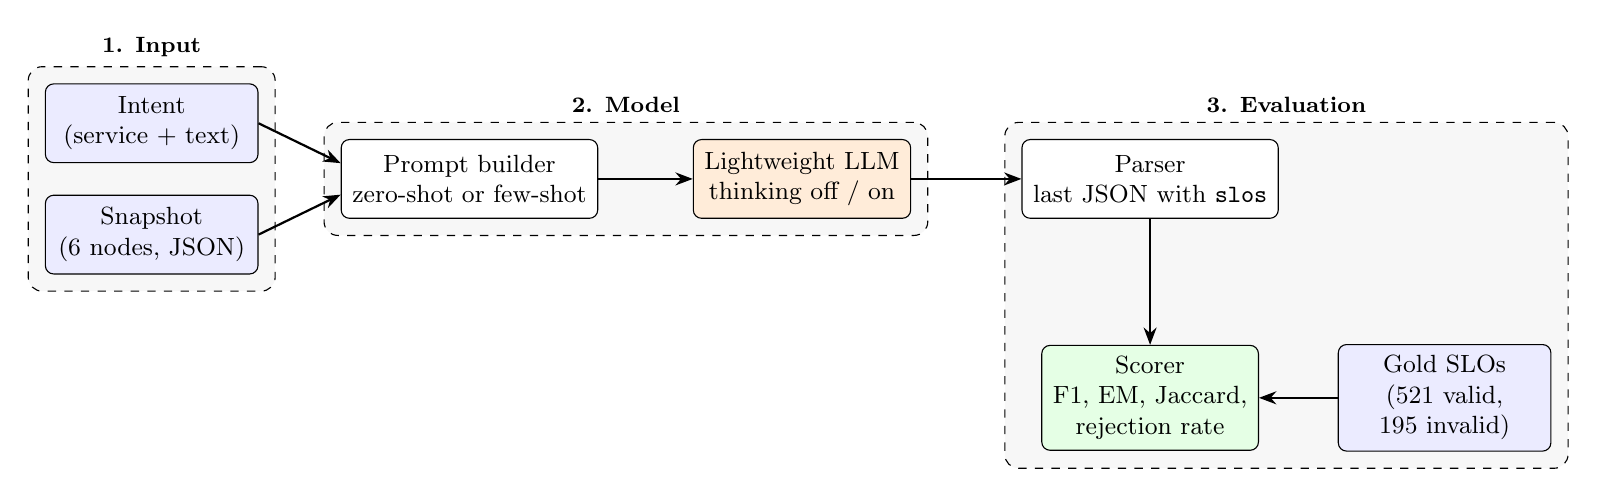
\begin{tikzpicture}[font=\small,
  box/.style={draw,rounded corners=3pt,align=center,minimum height=10mm,minimum width=27mm,inner sep=4pt,fill=white},
  grp/.style={draw,dashed,rounded corners=5pt,inner sep=6pt,fill=gray!6},
  arr/.style={-{Stealth[length=2.2mm]},thick}]
\node[box,fill=blue!8] (intent) {Intent\\(service + text)};
\node[box,fill=blue!8,below=4mm of intent] (snap) {Snapshot\\(6 nodes, JSON)};
\node[box,right=24mm of $(intent)!0.5!(snap)$] (prompt) {Prompt builder\\zero-shot or few-shot};
\node[box,fill=orange!15,right=12mm of prompt] (llm) {Lightweight LLM\\thinking off / on};
\node[box,right=14mm of llm] (parse) {Parser\\last JSON with \texttt{slos}};
\node[box,fill=green!10,below=16mm of parse] (score) {Scorer\\F1, EM, Jaccard,\\rejection rate};
\node[box,fill=blue!8,right=10mm of score] (gold) {Gold SLOs\\(521 valid,\\195 invalid)};
\begin{scope}[on background layer]
\node[grp,fit=(intent)(snap),label={[font=\footnotesize\bfseries]above:1. Input}] {};
\node[grp,fit=(prompt)(llm),label={[font=\footnotesize\bfseries]above:2. Model}] {};
\node[grp,fit=(parse)(score)(gold),label={[font=\footnotesize\bfseries]above:3. Evaluation}] {};
\end{scope}
\draw[arr] (intent.east) -- ($(prompt.west)+(0,2mm)$);
\draw[arr] (snap.east) -- ($(prompt.west)-(0,2mm)$);
\draw[arr] (prompt) -- (llm); \draw[arr] (llm) -- (parse);
\draw[arr] (parse) -- (score); \draw[arr] (gold) -- (score);
\end{tikzpicture}
\end{document}
